\documentclass{beamer}

\usepackage{tikz-uml}
\usepackage[T1]{fontenc}
\usepackage{listings}
\usepackage{amsmath}
\usepackage{verbatim}
\usepackage{tikz-uml}
\usepackage{ifthen}
\usetikzlibrary {automata,positioning}
\usepackage{xargs}
\newcommand{\semaut}[1]{[\![#1]\!]}
\newcommand{\sembox}[1]{
    #1
}
\newcommandx{\automaton}[7][1=, 2=Q, 3=C, 4=\Delta, 5=\Sigma, 6=s, 7=F]{
    (#2#1, #3#1, #4#1, #5, #6#1, #7#1)
}
\newcommandx{\transition}[6][1=, 2=q, 3=q', 4=\phi, 5=p, 6=a]{
    (#2#1, #4#1, #5#1, #6, #3#1)
}
\newcommandx{\clockreduction}[0]{
    \mathbb{C}_r
}
\newcommandx{\deadedge}[0]{
    \mathbb{T}_d
}
\newcommandx{\deadclock}[0]{
    \mathbb{C}_d
}
\newcommandx{\deadstate}[0]{
    \mathbb{S}_d
}
\newcommandx{\unreachable}[0]{
    \mathbb{S}_u
}
\newcommandx{\pruning}[0]{
    \mathbb{P}
}
\newcommandx{\str}[1]{
    \underline{#1}
}

\newcommandx{\plot}[8]{
    \begin{tikzpicture}
        \begin{semilogyaxis}[
                title={Mean Time},
                width=15cm,
                height=10cm,
                ymin=0,
                legend pos=north west,
                xlabel={Iterations},
                ylabel={Time(ns)},
                xtick={#1},
                ymajorgrids=true,
            ]

            \addplot[color=yellow, mark=square*] coordinates {#2};
            \addlegendentry{N}
            \addplot[color=gray, mark=square*] coordinates {#3};
            \addlegendentry{E}
            \addplot[color=red, mark=square*] coordinates {#4};
            \addlegendentry{S}
            \addplot[color=black, mark=square*] coordinates {#5};
            \addlegendentry{SS}
            \addplot[color=green, mark=square*] coordinates {#6};
            \addlegendentry{SE}
            \addplot[color=violet, mark=square*] coordinates {#7};
            \addlegendentry{ES}
            \addplot[color=blue, mark=square*] coordinates {#8};
            \addlegendentry{EE}
        \end{semilogyaxis}
    \end{tikzpicture}
}

\newcommandx{\plotmem}[8]{
    \begin{tikzpicture}
        \begin{semilogyaxis}[
                title={Allocated Memory},
                width=15cm,
                height=10cm,
                ymin=0,
                legend pos=north west,
                xlabel={Iterations},
                ylabel={Memory (kb)},
                xtick={#1},
                ymajorgrids=true,
            ]

            \addplot[color=yellow, mark=square*] coordinates {#2};
            \addlegendentry{N}
            \addplot[color=gray, mark=square*] coordinates {#3};
            \addlegendentry{E}
            \addplot[color=red, mark=square*] coordinates {#4};
            \addlegendentry{S}
            \addplot[color=black, mark=square*] coordinates {#5};
            \addlegendentry{SS}
            \addplot[color=green, mark=square*] coordinates {#6};
            \addlegendentry{SE}
            \addplot[color=violet, mark=square*] coordinates {#7};
            \addlegendentry{ES}
            \addplot[color=blue, mark=square*] coordinates {#8};
            \addlegendentry{EE}
        \end{semilogyaxis}
    \end{tikzpicture}
}
\newcommandx{\captionof}[2]{

}

\newcommand{\name}{}

\addtobeamertemplate{navigation symbols}{}{%
    \usebeamerfont{footline}%
    \usebeamercolor[fg]{footline}%
    \hspace{1em}%
    \name
    \hspace{1em}%
    \insertframenumber/\inserttotalframenumber
}

\usetheme{Frankfurt}
\useinnertheme{rectangles}
% \setbeamertemplate{footline}[frame number]


\title{TREAT}
\subtitle{Timed Regular Expression to Automaton Transformation}
\author{Group 30}
\institute{Aalborg Universitet}
\date{2024}

\begin{document}


\frame{\titlepage}

\begin{frame}{Agenda}
    \tableofcontents
\end{frame}

\section{Intro} % each section gets own category on top bar, each frame within gets a subcategory
\renewcommand{\name}{Marcus}
%Marcus Section

\begin{frame}{Introduction}
    \centering
    \LARGE\textbf{TREAT} \\
    \vspace{0.5cm}
    \Large\textit{Timed Regular Expression to Automaton Transformation}
\end{frame}

\section{Process}

\begin{frame}{Process}
    \begin{itemize}
        \item Initial Problem
        \item Pivot
        \item Human Readability and Usability
    \end{itemize}
\end{frame}

\begin{frame}{Process}
    \textbf{Initial Problem}

    ``Better Timed Pattern Searching in Log Files''
    \newline
    \begin{itemize}
        \item The paper: ``Timed Regular Expressions''
        \item What should the program contain?
              \begin{itemize}
                  \item Parse TREs
                  \item Convert TREs to timed automata
                  \item Perform checking (Output to UPPAAL)
              \end{itemize}
    \end{itemize}

    Can we output to UPPAAL in a better way?
\end{frame}

\begin{frame}{Process}
    \textbf{Pivot}

    We will still have the same features, but checking will take a lower priority.
    \newline
    \begin{itemize}
        \item Pruning
        \item Graphing
    \end{itemize}
\end{frame}

\begin{frame}{Process}
    \textbf{Human Readability and Usability}

    Focus on efficient transformation from TRE to TA.
    \newline
    \begin{itemize}
        \item TRE input improvement
              \begin{itemize}
                  \item Multi-character symbols
              \end{itemize}
        \item CLI
        \item TikZ
    \end{itemize}

    These could have been done regardless, but became a larger focus now.
\end{frame}

\section{Program}

\begin{frame}[shrink=5]{Implementation}
    \begin{center}
        \section{TREAT Diagram}\label{fig:TREATdiagram}
The following diagram shows the flow of data through the TREAT program. The diagram is meant as an overall outline, and is not supposed to be precise. 

\begin{tikzpicture}[node distance = 3cm, auto]
    \node (CLI) {CLI};
    \node (TimedWord) [below right of = CLI] {Timed Word};
    \node (TRE) [right of = CLI] {TRE};
    \node (Tokenizer) [right of = TRE] {Tokenizer};
    \node (TAGenerator) [right of = Tokenizer] {TA Generator};
    \node (Pruning) [right of = TAGenerator] {Pruning};
    \node (Graph) [right of = Pruning] {Graph};
    \node (Output) [below of = Graph] {Output};
    \node (UPPAAL) [below left of = Output] {UPPAAL};
    \node (XML) [below of = UPPAAL] {XML};
    \node (UPPAALAutomaton) [below of = XML] {UPPAAL Automaton};
    \node (TikZ) [below right of = Output] {TikZ};
    \node (TimedWordGenerator) [node distance = 7 cm, right of = TimedWord] {Timed Word Generator};

    \draw[->] (CLI) -- (TRE);
    \draw[->] (TRE) -- (Tokenizer);
    \draw[->] (Tokenizer) -- (TAGenerator);
    \draw[->] (TAGenerator) -- (Pruning);
    \draw[->] (Pruning) -- (Graph);
    \draw[->] (Graph) -- (Output);
    \draw[->] (Output) -- (UPPAAL);
    \draw[->] (UPPAAL) -- (XML);
    \draw[->] (XML) -- (UPPAALAutomaton);
    \draw[->] (Output) -- (TikZ);
    \draw[->] (CLI) -- (TimedWord);
    \draw[->] (TimedWord) -- (TimedWordGenerator);
    \draw[->] (TimedWordGenerator) -- (Output);
\end{tikzpicture}
    \end{center}
\end{frame}

\begin{frame}[shrink=20]{Parser}
    
\textbf{CFG}

TimedRegex := Match

\qquad	$\mid$ Parentheses

Parentheses := parenthesisStart Match parenthesisEnd

\qquad	$\mid$ Parentheses Binary Match

\qquad	$\mid$ Parentheses Unary

\qquad $\mid$ Parentheses Interval

Match := match Unary

\qquad	$\mid$ match Interval

\qquad    $\mid$ Match Binary match

\qquad	$\mid$ match

Interval := IntervalBoundry Number intervalSeperator Number IntervalBoundry

IntervalBoundry := intervalLeft

\qquad	$\mid$ intervalRight

Number := Number digit

\qquad	$\mid$ digit

Unary := iterator

\qquad	$\mid$ guranteedIterator

\qquad	$\mid$ AbsorbedIteration

\qquad	$\mid$ AbsorbedGuranteedIterator

\qquad	$\mid$ Rename

Binary := union

\qquad	$\mid$ concatenation

\qquad	$\mid$ intersection

\qquad	$\mid$ AbsorbedConcatenation

AbsorbedGuranteedIterator := guranteedIterator absorb 

AbsorbedConcatenation := absorb concatenation

AbsorbedIteration := iterator absorb 

Rename := renameStart leftCurlyBrace RenameSymbols rightCurlyBrace

RenameSymbols := match match

\qquad	$\mid$ match match comma RenameSymbols
\end{frame}

\begin{frame}{Parser}
    \scalebox{0.8}{\begin{tikzpicture}
    %interfaces
    \umlclass[x=0,y=-3]{IAstNode}{token: Token}{}

    %classes
    \umlclass[x=0,y=-6]{IBinary}{left: IAstNode}{right: IAstNode}
    \umlclass[x=3.5,y=-6]{IUnary}{child: IAstNode}{}
    \umlclass[x=6.5,y=-6]{Match}{}{}
    %\umlclass[anchor=north,x=1,y=-9]{Interval}{startInterval: int\\endInterval: int\\startInclusive: bool\\endInclusive: bool}{}
    %\umlclass[anchor=north,x=6,y=-9]{Rename}{renameSymbols: symbolReplace[]}{}
    \umlclass[x=9,y=-6]{Epsilon}{}{}
    \umlsimpleclass[x=3.5,y=-8,draw=none,fill=none,alias=unarydots,scale=2]{...}
    \umlsimpleclass[x=3.5,y=-8,fill=none,draw=none,alias=phantomunary]{ }
    \umlsimpleclass[x=0,y=-8,fill=none,draw=none,scale=2]{...}
    \umlsimpleclass[x=0,y=-8,fill=none,draw=none,alias=phantombinary]{ }

    % \umlclass[anchor=north,x=9,y=-12]{AbsorbedConcatenation}{}{}
    % \umlclass[anchor=north,x=12,y=-12]{AbsorbedGuaranteedIterator}{}{}
    % \umlclass[anchor=north,x=15,y=-12]{AbsorbedIterator}{}{}
    % \umlclass[anchor=north,x=18,y=-12]{Concatenation}{}{}
    % \umlclass[anchor=north,x=21,y=-12]{GuaranteedIterator}{}{}
    % \umlclass[anchor=north,x=27,y=-12]{Intersection}{}{}
    % \umlclass[anchor=north,x=6,y=-12]{Interval}{}{}
    % \umlclass[anchor=north,x=3,y=-12]{Iterator}{}{}
    % \umlclass[anchor=north,x=0,y=-12]{Union}{}{}
    

    %transitions
    \umlVHVinherit[arm1=1.5cm]{IUnary}{IAstNode}
    \umlVHVinherit[]{IBinary}{IAstNode}
    \umlVHVinherit[arm1=1.5cm]{Match}{IAstNode}
    \umlVHVinherit[arm1=1.5cm]{Epsilon}{IAstNode}
    \umlVHVinherit[arm1=0.5cm]{phantomunary}{IUnary}
    \umlVHVinherit[arm1=0.5cm]{phantombinary}{IBinary}

    \umlcompo[anchor1=120,anchor2=east,arg1=1,arg2=1,geometry=|-,pos2=1.8]{IUnary}{IAstNode}
    %\umlcompo[arg1=2,arg2=1]{IBinary}{IAstNode}
    \umlCNassoc[arg1=2]{IAstNode}{-3,-3}{-3,-6}
    \umlCNcompo[arg1=1]{IBinary}{-3,-6}{-3,-6}

    % \umlaggreg[attr1=1|,attr2=2|]{IBinary}{IAstNode}

    % \umlVHVinherit[]{Interval}{IUnary}
    % \umlVHVinherit[]{Rename}{IUnary}

    %\draw [tikzuml aggregation style] (IUnary.-120)-- ++(0cm,-1cm)node[pos=0.2, left]{1} -- ++(-4.5cm,0cm) |- (IAstNode.west)node[pos=0.8, below]{1};

\end{tikzpicture}}
\end{frame}

\begin{frame}{TA UML}
    \begin{tikzpicture}
    \umlclass{TA}{alphabet: Set<string>\\finalStates: Set<State>\\initial: State}
    {ReduceClocks()\\PruneEdges()\\PruneDeadStates()\\PruneUnreachableStates()\\PruneClocks()}
    
    \umlclass[x=-4, y=-6]{State}{id: int\\x,y: int\\}{}
    \umlcompo[geometry=-|,attr1=0..*|,attr2=1|,pos1=1.8,pos2=0.2]{TA}{State}
    
    \umlclass[y=-6]{Transition}{id: int\\ranges: Set<(Range,Clock)>\\reset: Set<Clock>}{}
    \umlcompo[geometry=|-|,attr1=|0..*,attr2=1|,pos1=1.8,pos2=0.2]{TA}{Transition}
    
    \umlclass[x=4,y=-6]{Clock}{id: int}{}
    \umlcompo[geometry=-|,attr1=0..*|,attr2=1|,pos1=1.8,pos2=0.2]{TA}{Clock}
    
\end{tikzpicture}
\end{frame}

%End of Marcus section

\renewcommand{\name}{Frederik}
% =======================================================================
% Semantics
% =======================================================================

\section{Semantics}
\begin{frame}[fragile]{Match semantics}
    Assarin et al.

    \textit{The automaton for \underline{$[\![a]\!]$}}, $a\in\Sigma$ is $(\{s,f\},\emptyset,\Delta,\Sigma,s,\{f\})$ where the transition relation is $\Delta={(s,true,\emptyset,a,f)}$.
    
    \begin{lstlisting}[language=c++,basicstyle=\small]
void Visit(Match match)
{
    TimedAutomaton ta = new(_regex);
    
    State initial = ta.AddState(newInitial: true);
    State final = ta.AddState(true);

    ta.AddEdge(initial, final, match.Token.Match);

    _stack.Push(ta);
}
    \end{lstlisting}
\end{frame}

\begin{frame}{Union semantics}
    Assarin et al.

    \textit{The automaton for $[[\varphi_1\vee\varphi_2]]$ is $(Q_1\cup Q_2 \cup \{s\},C_1\cup C_2,\Delta,\Sigma,s,F_1\cup F_2)$, where $\Delta$ is constructed
by adding to $\Delta_1\cup \Delta_2$ two new $\epsilon$-transitions $(s, x = 0,\emptyset,\epsilon,s_i)$, where $x$ is any clock and $i\in{1,2}$
(if there is no clock in the automata we should add one).}

\usetikzlibrary {automata,positioning}
% "A|B"
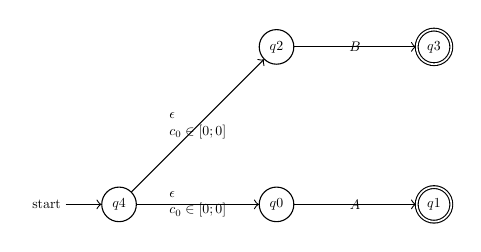
\begin{tikzpicture}[every node/.style={scale=0.5}]
    \node[state] at (2, 0)(q0){$q0$};
    \node[state, accepting] at (4, 0)(q1){$q1$};
    \node[state] at (2, 2)(q2){$q2$};
    \node[state, accepting] at (4, 2)(q3){$q3$};
    \node[state, initial] at (0, 0)(q4){$q4$};
    
    \path[->]
        (q0)edge node[align=left]{$A$}(q1)
        (q2)edge node[align=left]{$B$}(q3)
        (q4)edge node[align=left]{$\epsilon$\\$c_0\in[0;0]$}(q0)
        (q4)edge node[align=left]{$\epsilon$\\$c_0\in[0;0]$}(q2)
        ;
\end{tikzpicture}

% "A|B"
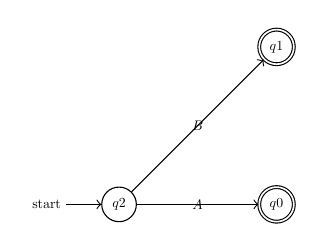
\begin{tikzpicture}[every node/.style={scale=0.5}]
    \node[state, accepting] at (2, 0)(q0){$q0$};
    \node[state, accepting] at (2, 2)(q1){$q1$};
    \node[state, initial] at (0, 0)(q2){$q2$};
    
    \path[->]
        (q2)edge node[align=left]{$A$}(q0)
        (q2)edge node[align=left]{$B$}(q1)
        ;
\end{tikzpicture}
\end{frame}

\begin{frame}{Union semantics revised}
    $\bracket[\varphi_1\vee\varphi_2]=\left\{\begin{array}{ll}
    \bracket[(\epsilon\cdot\varphi_1)\cup\varphi_2] & if (q_1,\phi_1,p_1,a,s_1)\in\Delta_1 \\
    \bracket[\varphi_1\cup(\epsilon\cdot\varphi_2)] & if (q_2,\phi_2,p_2,a,s_2)\in\Delta_2 \\
    (Q_1\cup Q_2 \cup {s}\backslash\{s_1,s_2\},C_1\cup C_2,\Delta,\Sigma,s,F_1\cup F_2\backslash\{s_1,s_2\}) & otherwise \\
    \end{array}\right.
    $
    
    Where
    
    $\Delta_e=\{(q,\phi,p,a,q')|
    (q,\phi,p,a,q')\in\Delta_1\wedge q\neq s_1
    \vee
    (q,\phi,p,a,q')\in\Delta_2\wedge q\neq s_2\}$

    $\Delta_s=\{(s,\phi,p,a,q')|
    \exists. q (q,\phi,p,a,q')\in\Delta_1
    \vee    q (q,\phi,p,a,q')\in\Delta_2\}$

    $\Delta=\Delta_e\cup\Delta_s$
    \newline

    $\forall (q_1,\phi_1,p_1,a,q_1')\in\Delta_1\wedge q_1\neq s_1 \implies (q_1,\phi_1,p_1,a,q_1')\in\Delta$
    
    $\forall (q_2,\phi_2,p_2,a,q_2')\in\Delta_2\wedge q_2\neq s_2 \implies (q_2,\phi_2,p_2,a,q_2')\in\Delta$
    
    $\forall (s_1,\phi_1,p_1,a,q_1')\in\Delta_1\implies (s,\phi_1,p_1,a,q_1')\in\Delta$
    
    $\forall (s_2,\phi_2,p_2,a,q_2')\in\Delta_2\implies (s,\phi_2,p_2,a,q_2')\in\Delta$
\end{frame}

\begin{frame}[fragile]{Union implementation}
    \begin{lstlisting}[language=c++,basicstyle=\tiny]
(TimedAutomaton right, TimedAutomaton left) = (_stack.Pop(), _stack.Pop());
EpsilonConcat(right);
EpsilonConcat(left);
TimedAutomaton ta = new(left, right, e => IsNotInitial(e.From), IsNotInitial);

State initial = ta.AddState(newInitial: true);

foreach (Edge edges in left.GetEdgesFrom(left.InitialState!)
    .Concat(right.GetEdgesFrom(right.InitialState!)))
{
    Edge e = ta.AddEdge(initial, edges.To, edges.Symbol);
    e.AddClockRanges(edges.GetClockRanges());
    e.AddClockResets(edges.GetClockResets());
}

static void EpsilonConcat(TimedAutomaton ta)
{
    if (ta.GetEdgesTo(ta.InitialState!).Any())
    {
        State oldInitial = ta.InitialState!;
        State newInitial = ta.AddState(ta.IsFinal(oldInitial), true);
        Edge edge = ta.AddEdge(newInitial, oldInitial, "\0");
    }
}
    \end{lstlisting}
\end{frame}

\begin{frame}[fragile]{Lazy intersection}
    Lazily generate new states
    \begin{lstlisting}[basicstyle=\tiny]
State GetNewState(State lState, State rState)
{
    if (!newLocs.TryGetValue((lState, rState), out State? state))
    {
        state = ta.AddState();
        newLocs[(lState, rState)] = state;
    }

    return state;
}
    \end{lstlisting}
\end{frame}

% =======================================================================
% Timed word generator
% =======================================================================
\section{Timed words}
\begin{frame}[fragile]{Timed word generation}
    \begin{columns}
        \begin{column}{0.5\textwidth}
            nasa.gov
            \begin{lstlisting}[basicstyle=\tiny]
00 00 00 04 CDR
Roger. Clock.

00 00 00 13 CDR
Roger. We got a roll program.

00 00 00 15 CMP
Roger. Roll.

00 00 00 34 CDR
Roll's complete and the pitch is programed.

00 00 00 44 CDR
One Bravo.

00 00 01 02 CC
Apollo 11, Houston. You're good at 1 minute.
...
            \end{lstlisting}
        \end{column}
        \begin{column}{0.5\textwidth}
            apollo11transcript.csv
            \begin{lstlisting}[basicstyle=\tiny]
CDR, 4


CDR, 13


CMP, 15


CDR, 34


CDR, 44


CC, 62

...
            \end{lstlisting}
        \end{column}
    \end{columns}
\end{frame}

\begin{frame}[fragile]{Words as timed automata.}
    In Uppaal
    \begin{columns}
        \begin{column}{0.5\textwidth}
            % "(<CDR>|<CC>|<CMP>)+"
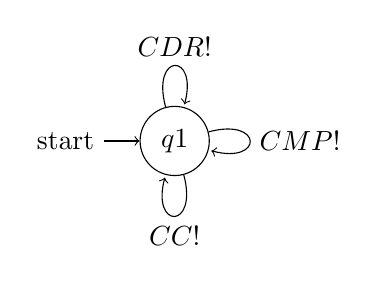
\begin{tikzpicture}[auto]
    \node[state, initial] at (0, 0)(q1){$q1$};
    
    \path[->]
        (q1)edge [loop above] node[align=left]{$CDR!$}(q1)
        (q1)edge [loop below] node[align=left]{$CC!$}(q1)
        (q1)edge [loop right] node[align=left]{$CMP!$}(q1)
        ;
\end{tikzpicture}
            
        \end{column}
        \begin{column}{0.5\textwidth}
            \begin{lstlisting}[basicstyle=\tiny]
update: index++
guard: index <= 8439 &&
    word[index] == "" &&
    times[index] == "CDR"
            \end{lstlisting}
        \end{column}
    \end{columns}
    \begin{lstlisting}[basicstyle=\tiny]
clock c0;
int32_t index = 0;
const string word[8439] = {"CDR", "CDR", "CMP", "CDR", "CDR", "CC", ... }
clock_t times[8439] = {4, 13, 15, 34, 44, 62, ... }
    \end{lstlisting}
\end{frame}

% =======================================================================
% Pruning
% =======================================================================
\section{Pruning}
\newcommandx{\captionof}[2]{

}
\begin{frame}{Example}
    $$C(A[5;10]\&(BA|A)[1;3])$$
    % Generated by: TimedRegex, Version = 1.0.0.0
% Date 5/12/2024 10:20:04 PM
\usetikzlibrary {automata,positioning}
% "A[1;1]+'"
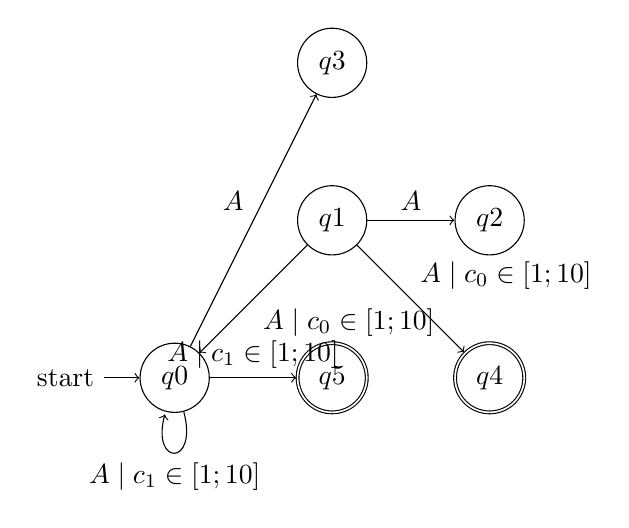
\begin{tikzpicture}[auto]
    \node[state, initial] at (0, 0)(q0){$q0$};
    \node[state] at (2, 2)(q1){$q1$};
    \node[state] at (4, 2)(q2){$q2$};
    \node[state] at (2, 4)(q3){$q3$};
    \node[state, accepting] at (4, 0)(q4){$q4$};
    \node[state, accepting] at (2, 0)(q5){$q5$};
    
    \path[->]
        (q1)edge node{$A$}(q2)
        (q0)edge node{$A$}(q3)
        (q1)edge node{$A\mid c_0\in[1;10]$}(q4)
        (q1)edge node{$A\mid c_0\in[1;10]$}(q0)
        (q0)edge node{$A\mid c_1\in[1;10]$}(q5)
        (q0)edge [loop below] node{$A\mid c_1\in[1;10]$}(q0)
        ;
    \label{fig:prune0}
\end{tikzpicture}
 

\end{frame}
\begin{frame}{Clock reduction}
    Daws et al.
    \input{Automata/Prune1.tex}
\end{frame}
\begin{frame}{Dead transition}
    \begin{definition}\label{definition:deadEdgePruning}
    Dead edge pruning:
    \sembox{
        $\deadedge(A)=\automaton[][Q][C][\Delta'][\Sigma][s][F]$
    
        $\Delta'=\{\transition\in\Delta\mid\phi\neq\emptyset\wedge\emptyset\neq\cap_{i=1}^n\phi_i\}$
    }
\end{definition}
    \input{Automata/Prune2.tex}
\end{frame}
\begin{frame}{Unreachable state}
    % Unreachable states are very similar to dead states.
% Except we check for any edges that end at a given state.
% If a state is not reachable it is removed.
% Repeat until no such states exist.
\begin{definition}\label{definition:unreachableStatePruning}
    Unreachable state pruning:

    \sembox{
        $\unreachable\automaton=\automaton[][Q'][C][\Delta'][\Sigma][s][F']$

        $U(q')=q'\neq s \wedge\nexists\transition\in\Delta$

        $Q'=\{q\in Q\mid \neg U(q)\}$

        $\Delta'=\{\transition[]\in\Delta\mid q'\in Q'\}$

        $F'=F\cap Q'$
    }
\end{definition}
    % Generated by: TimedRegex, Version = 1.0.0.0
% Date 5/14/2024 6:44:16 PM
\usetikzlibrary {automata,positioning}
% "C(A[5;10]&(BA|A)[1;3])"
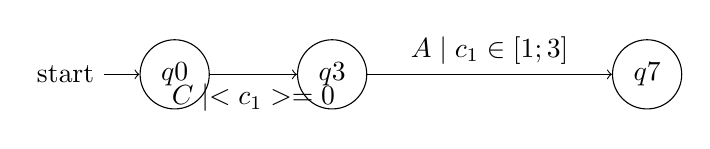
\begin{tikzpicture}[auto]
    \node[state, initial] at (0, 0)(q0){$q0$};
    \node[state] at (2, 0)(q3){$q3$};
    \node[state] at (6, 0)(q7){$q7$};
    
    \path[->]
        (q3)edge node[above]{$A\mid c_1\in[1;3]$}(q7)
        (q0)edge node[below]{$C\mid <c_1>=0$}(q3)
        ;
\end{tikzpicture}
 

\end{frame}
\begin{frame}{Dead state}
    %Dead states are all the states that have no way of reaching the final state.
%These states are pruned by removing all states that have no edges away from them unless they are final states, this is repeated until no states satisfy this property.
\begin{definition}\label{definition:deadStatePruning}
    Dead state pruning:
    
    \sembox{
        $\deadstate(A_1)=\left\{\begin{array}{ll}
            A_1 & if \forall q\in Q_1:\neg D(q) \\
            \deadstate(\automaton[][Q][C_1][\Delta][\Sigma_1][s_1][F_1]) & otherwise \\
        \end{array}\right.
        $

        $D(q)=q\notin F_1\wedge \transition[_1]\notin\Delta_1$

        $Q=\{q\in Q_1\mid\neg D(q)\}$

        $\Delta=\{\transition[_1]\in\Delta_1\mid q_1\in Q\}$
    }
\end{definition}
    % Generated by: TimedRegex, Version = 1.0.0.0
% Date 5/14/2024 6:44:16 PM
\usetikzlibrary {automata,positioning}
\scalebox{0.9}{
    % "C(A[5;10]&(BA|A)[1;3])"
    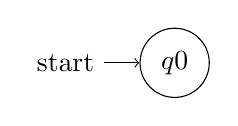
\begin{tikzpicture}[auto]
        \node[state, initial] at (0, 0)(q0){$q0$};
        
        \path[->]
            ;
    \end{tikzpicture}
}

\captionof{figure}{Dead state $q7$ has been removed.}
\label{fig:prune4}

\end{frame}
\begin{frame}{Dead clock}
    % Any clocks that are not used in any intervals can be removed.
% This means removing them both from the clocks set and from any clock resets.
% This shouldn't have a huge impact, but it will allow us to create a more minimal declaration field in Uppaal.
\begin{definition}\label{definition:deadClockPruning}
    Dead clock pruning:
    
    \sembox{
        $\deadclock(A_1)=\automaton[][Q_1][C][\Delta][\Sigma_1][s_1][F_1]$
        
        $C=\{c\mid\exists\transition[_1]\in\Delta_1:\langle c\in I\rangle\in\phi_1\}$

        $\Delta=\{\transition[][q_1][q_1'][\phi_1][p\backslash C]\mid\transition[_1]\in\Delta_1\}$
    }
\end{definition}
    \input{Automata/Prune5.tex}
\end{frame}
\begin{frame}{Recursion}
    \begin{definition}\label{definition:recursivePruning}
    Recursive pruning:
    
    \sembox{
        $\pruning(A)=\left\{\begin{array}{ll}
            A & \text{if }A=A' \\
        \pruning(A') & otherwise \\
        \end{array}\right.
        $

        $A' = \clockreduction\circ\deadedge\circ\deadstate\circ\unreachable\circ\deadclock(A)$
    }
\end{definition}
    % Generated by: TimedRegex, Version = 1.0.0.0
% Date 5/14/2024 6:44:16 PM
\usetikzlibrary {automata,positioning}
\scalebox{0.9}{
    % "C(A[5;10]&(BA|A)[1;3])"
    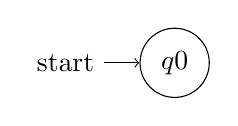
\begin{tikzpicture}[auto]
        \node[state, initial] at (0, 0)(q0){$q0$};
    \end{tikzpicture}
}

\captionof{figure}{Final pruned automaton.}
\label{fig:prune6}

\end{frame}

\begin{frame}
    \begin{definition}\label{definition:recursivePruning}
    Recursive pruning:
    
    \sembox{
        $\pruning(A)=\left\{\begin{array}{ll}
            A & \text{if }A=A' \\
        \pruning(A') & otherwise \\
        \end{array}\right.
        $

        $A' = \clockreduction\circ\deadedge\circ\deadstate\circ\unreachable\circ\deadclock(A)$
    }
\end{definition}
    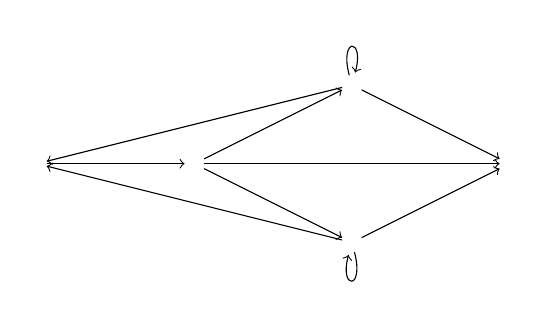
\begin{tikzpicture}[auto]
    \node[] at (0, 0)(cr){$\clockreduction$};
    \node[] at (4, -1)(sd){$\deadstate$};
    \node[] at (4, 1)(su){$\unreachable$};
    \node[] at (2, 0)(td){$\deadedge$};
    \node[] at (6, 0)(cd){$\deadclock$};
    
    \path[->]
        (su)edge [loop above] node{}(su)
        (sd)edge [loop below] node{}(sd)
        (su)edge node[align=left]{}(cr)
        (sd)edge node[align=left]{}(cr)
        (td)edge node[align=left]{}(sd)
        (td)edge node[align=left]{}(su)
        (sd)edge node[align=left]{}(cd)
        (su)edge node[align=left]{}(cd)
        (td)edge node[align=left]{}(cd)
        (cr)edge node[align=left]{}(td)
        ;
\end{tikzpicture}
\end{frame}

% =======================================================================
% Graph layout
% =======================================================================
\section{Graph layout}
\begin{frame}
    We dont need precise algorithm
    \begin{itemize}
        \item Make graph acyclic (trivial)
        \item Assign states to layers
        \item Order states in layers (just needs to be good enough)
        \item Assign positions (simplicity over correctness)
    \end{itemize}
\end{frame}

\begin{frame}[fragile]{Creation of recursive edges}
    In automaton generator visitor
    \begin{lstlisting}[language=c++,basicstyle=\tiny]
public void Visit(GuaranteedIterator guaranteedIterator)
{
    TimedAutomaton ta = _stack.Pop();

    foreach (Edge oldEdge in ta.GetEdgesTo(ta.GetFinalStates()).ToList())
    {
        Edge edge = ta.AddEdge(oldEdge.From, ta.InitialState!, oldEdge.Symbol, true);
        edge.AddClockRanges(oldEdge.GetClockRanges());
        edge.AddClockResets(ta.GetClocks());
    }

    _stack.Push(ta);
}
    \end{lstlisting}
    \begin{lstlisting}[language=c++,basicstyle=\tiny]
public void Visit(AbsorbedGuaranteedIterator absorbedGuaranteedIterator)
    ...
    foreach (Edge childEdge in child.GetEdges())
        ...
        foreach (SortedSet<Clock> clockSet in clockPowerSet)
            ...    
            if (child.IsFinal(childEdge.To))
            {
                edge = ta.AddEdge(from, ta.InitialState!, childEdge.Symbol, true);
                edge.AddClockResets(childEdge.GetClockResets());
                edge.AddClockRanges(ranges);
            }
            ...
        ...
    ...
    \end{lstlisting}
\end{frame}

\begin{frame}[fragile]{Keeping reversible edges}
    In automaton generator visitor
    \begin{lstlisting}[language=c++,basicstyle=\tiny]
public void Visit(AbsorbedGuaranteedIterator absorbedGuaranteedIterator)
...
foreach (Edge childEdge in child.GetEdges())
    ...
    foreach (SortedSet<Clock> clockSet in clockPowerSet)
        ...
        Edge edge = ta.AddEdge(from, to, childEdge.Symbol, childEdge.IsReversible);
        edge.AddClockResets(childEdge.GetClockResets());
        edge.AddClockRanges(ranges);
        ...
    ...
...
    \end{lstlisting}
    
    \begin{lstlisting}[language=c++,basicstyle=\tiny]
public void Visit(Intersection intersection)
...
foreach (Edge lEdge in lEdges)
    ...
    foreach (Edge rEdge in rEdges)
        ...
        State from = GetNewEdge(lEdge.From, rEdge.From);
        State to = GetNewEdge(lEdge.To, rEdge.To);
        Edge edge = ta.AddEdge(from, to, c, lEdge.IsReversible || rEdge.IsReversible);
        edge.AddClockRanges(lEdge.GetClockRanges().Concat(rEdge.GetClockRanges()));
        edge.AddClockResets(lEdge.GetClockResets().Concat(rEdge.GetClockResets()));
        ...
    ...
...
    \end{lstlisting}
\end{frame}

\begin{frame}[fragile]{Removing recursive edges}
    In graphlayout
    \begin{lstlisting}[language=c++,basicstyle=\tiny]
private void AssignLayers(TimedAutomaton ta, TaState taState, int layerIndex)
...
foreach (Edge edge in ta.GetEdgesFrom(taState)
    .Where(e => !e.IsReversible))
    ...
foreach (Edge edge in ta.GetEdgesTo(taState)
    .Where(e => e.IsReversible && !e.To.Equals(taState)))
    ...
...
    \end{lstlisting}
\end{frame}

\renewcommand{\name}{Emil}
\section{Implementation}
\begin{frame}{UPPAAL}
    \begin{columns}
        \begin{column}{0.4\textwidth}
            \begin{itemize}
                \item UML
                \item Structured using UPPAAL .dtd
            \end{itemize}
        \end{column}
        \begin{column}{0.6\textwidth}
            \scalebox{0.8}{
                \scalebox{0.5}{\begin{tikzpicture}
        \umlclass[anchor=north,width=31ex,x=0,y=0]{nta}{system : string}{}

        %classes
        \umlclass[anchor=north,width=31ex,x=0,y=-4.3]{template}{name : string\\ init : string}{}
        \umlclass[anchor=north,width=31ex,x=-6,y=-9]{declaration}{clocks : list<string>\\channels : list<char>}{}

        %relations
        \umlcompo[attr1=1|,attr2=1..*|,pos2=0.87]{nta}{template}
        \umlHVcompo[attr1=1|,attr2=1|,pos1=0.1,pos2=1.98]{nta}{declaration}
        \umlHVcompo[attr1=1|,pos1=0.1,pos2=1.98]{template}{declaration}

        %classes
        %\umlclass[x=-6,y=-6]{parameter}{}{}
        %\umlclass[x=-3,y=-6]{branchpoint}{}{}
        \umlclass[anchor=north,width=31ex,x=0,y=-9]{location}{id : string\\name : string}{}
        \umlclass[anchor=north,width=31ex,x=6,y=-9]{transition}{source : string\\target : string}{}
        %\umlclass[x=15,y=-6]{parameter}{}{}
        %relations
        \umlcompo[attr1=1|,attr2=0..*|,pos1=0.15,pos2=0.9]{template}{location}
        \umlHVcompo[attr1=1|,attr2=0..*|,pos1=0.1,pos2=1.95]{template}{transition}
        %\umlVHVcompo[attr2=0..1|,pos2=2.75]{template}{parameter}

        %classes
        \umlclass[anchor=north,width=31ex,x=0,y=-14]{label}{kind : string\\ content : string}{}
        %relations
        \umlcompo[arg1=1,arg2=0..*,pos1=0.15,pos2=0.9]{location}{label}
        \umlVHcompo[arg1=1,arg2=0..*,pos1=0.1,pos2=1.9]{transition}{label}

        %classes
        %\umlclass[x=-6,y=-9]{committed}{}{}
        %\umlclass[x=-9,y=-9]{urgent}{}{}
        %relationsde
        %\umlVHVcompo[attr2=0..1|,pos2=2.75]{location}{committed}
        %\umlVHVcompo[attr2=0..1|,pos2=2.75]{location}{urgent}
    \end{tikzpicture}}


            }
        \end{column}
    \end{columns}
    % \hspace{10em}

\end{frame}
\begin{frame}[fragile]{UPPAAL}
    \definecolor{bluekeywords}{rgb}{0,0,1}
    \definecolor{greencomments}{rgb}{0,0.5,0}
    \definecolor{redstrings}{rgb}{0.64,0.08,0.08}
    \definecolor{xmlcomments}{rgb}{0.5,0.5,0.5}
    \definecolor{types}{rgb}{0.17,0.57,0.68}

    \lstset{language=[Sharp]C,
        captionpos=b,
        %numbers=left, %Nummerierung
        %numberstyle=\tiny, % kleine Zeilennummern
        frame=lines, % Oberhalb und unterhalb des Listings ist eine Linie
        showspaces=false,
        showtabs=false,
        breaklines=true,
        showstringspaces=false,
        breakatwhitespace=true,
        commentstyle=\color{greencomments},
        morekeywords={partial, var, value, get, set},
        keywordstyle=\color{bluekeywords},
        stringstyle=\color{redstrings},
        basicstyle=\ttfamily\tiny,
    }
    \begin{lstlisting}
internal Nta()
{
    _templates = new List<Template>();
    Declaration = new Declaration(new List<string>(), new List<string>());
}    
    \end{lstlisting}
    \vspace{1em}
    \begin{lstlisting}
internal Template(...)
{
    Declaration = declaration;
    Declaration.AddClocks(clocks);
    Name = name;
    Init = init;
    _locations = locations.ToArray();
    _transitions = transitions.ToArray();
}  
    \end{lstlisting}
\end{frame}

\begin{frame}{Demonstration}

\end{frame}

\section{Discussion}
\begin{frame}{Future works}
    \begin{columns}
        \begin{column}{0.4\textwidth}
            \begin{itemize}
                \item Pruning
                \item <4>TA $\rightarrow$ TRE
            \end{itemize}
        \end{column}
        \begin{column}{0.6\textwidth}
            \visible<2-3> {
                \scalebox{0.8}{
                    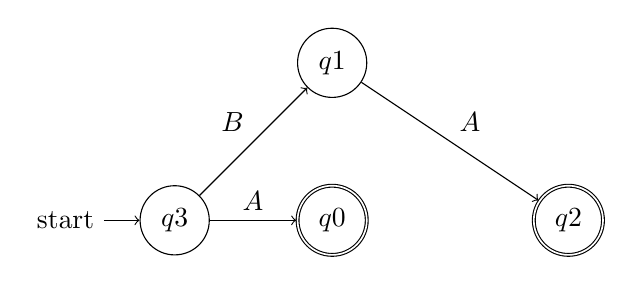
\begin{tikzpicture}[auto]
                        \node[state, accepting] at (2, 0)(q0){$q0$};
                        \node[state] at (2, 2)(q1){$q1$};
                        \node[state, accepting] at (5, 0)(q2){$q2$};
                        \node[state, initial] at (0, 0)(q3){$q3$};

                        \path[->]
                        (q1)edge node{$A$}(q2)
                        (q3)edge node{$A$}(q0)
                        (q3)edge node{$B$}(q1)
                        ;
                    \end{tikzpicture}
                }
            }

            \vspace{2em}
            \visible<3> {
                \scalebox{0.8}{
                    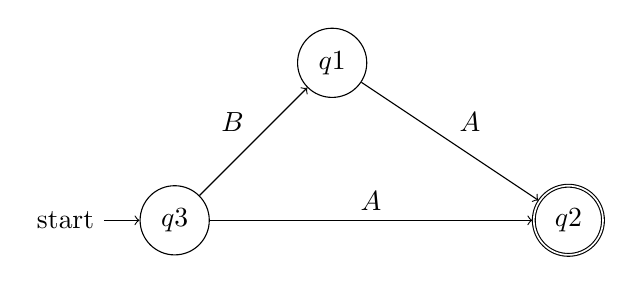
\begin{tikzpicture}[auto]
                        \node[state, accepting] at (5, 0)(q2){$q2$};
                        \node[state] at (2, 2)(q1){$q1$};
                        \node[state, initial] at (0, 0)(q3){$q3$};

                        \path[->]
                        (q1)edge node{$A$}(q2)
                        (q3)edge node{$A$}(q2)
                        (q3)edge node{$B$}(q1)
                        ;
                    \end{tikzpicture}
                }
            }
        \end{column}
    \end{columns}
\end{frame}
\begin{frame}{Enhancements}
    \begin{itemize}
        \item Bugfixes after hand-in
              \begin{itemize}
                  \item int32 indices
                  \item graph layout crashes
                  \item $\cdots$
              \end{itemize}
    \end{itemize}

\end{frame}
\begin{frame}{Learning Goals}
    \begin{itemize}
        \item is this relevant? genuine question
    \end{itemize}
\end{frame}
\section{Conclusion}
\begin{frame}{Conclusion}
    \begin{itemize}
        \item TREAT
        \item Readability
    \end{itemize}
\end{frame}

\end{document}